\documentclass[../../main/thesis_msc.tex]{subfiles}


\begin{document}

	\chapter{Results}
	
		
		
			\section{Single helium stars}
			
				\subsection{Internal structure - Core growth}
				
					\subsubsection{Evolution in the mass range $2.0$ M$_{\odot}$ to $2.8$ M$_{\odot}$}
					
					\subsubsection{Evolution in the mass range $2.9$ M$_{\odot}$ and above}
				
				
				\subsection{Radius evolution}
					
				
					\begin{figure}[h]
						\centering
						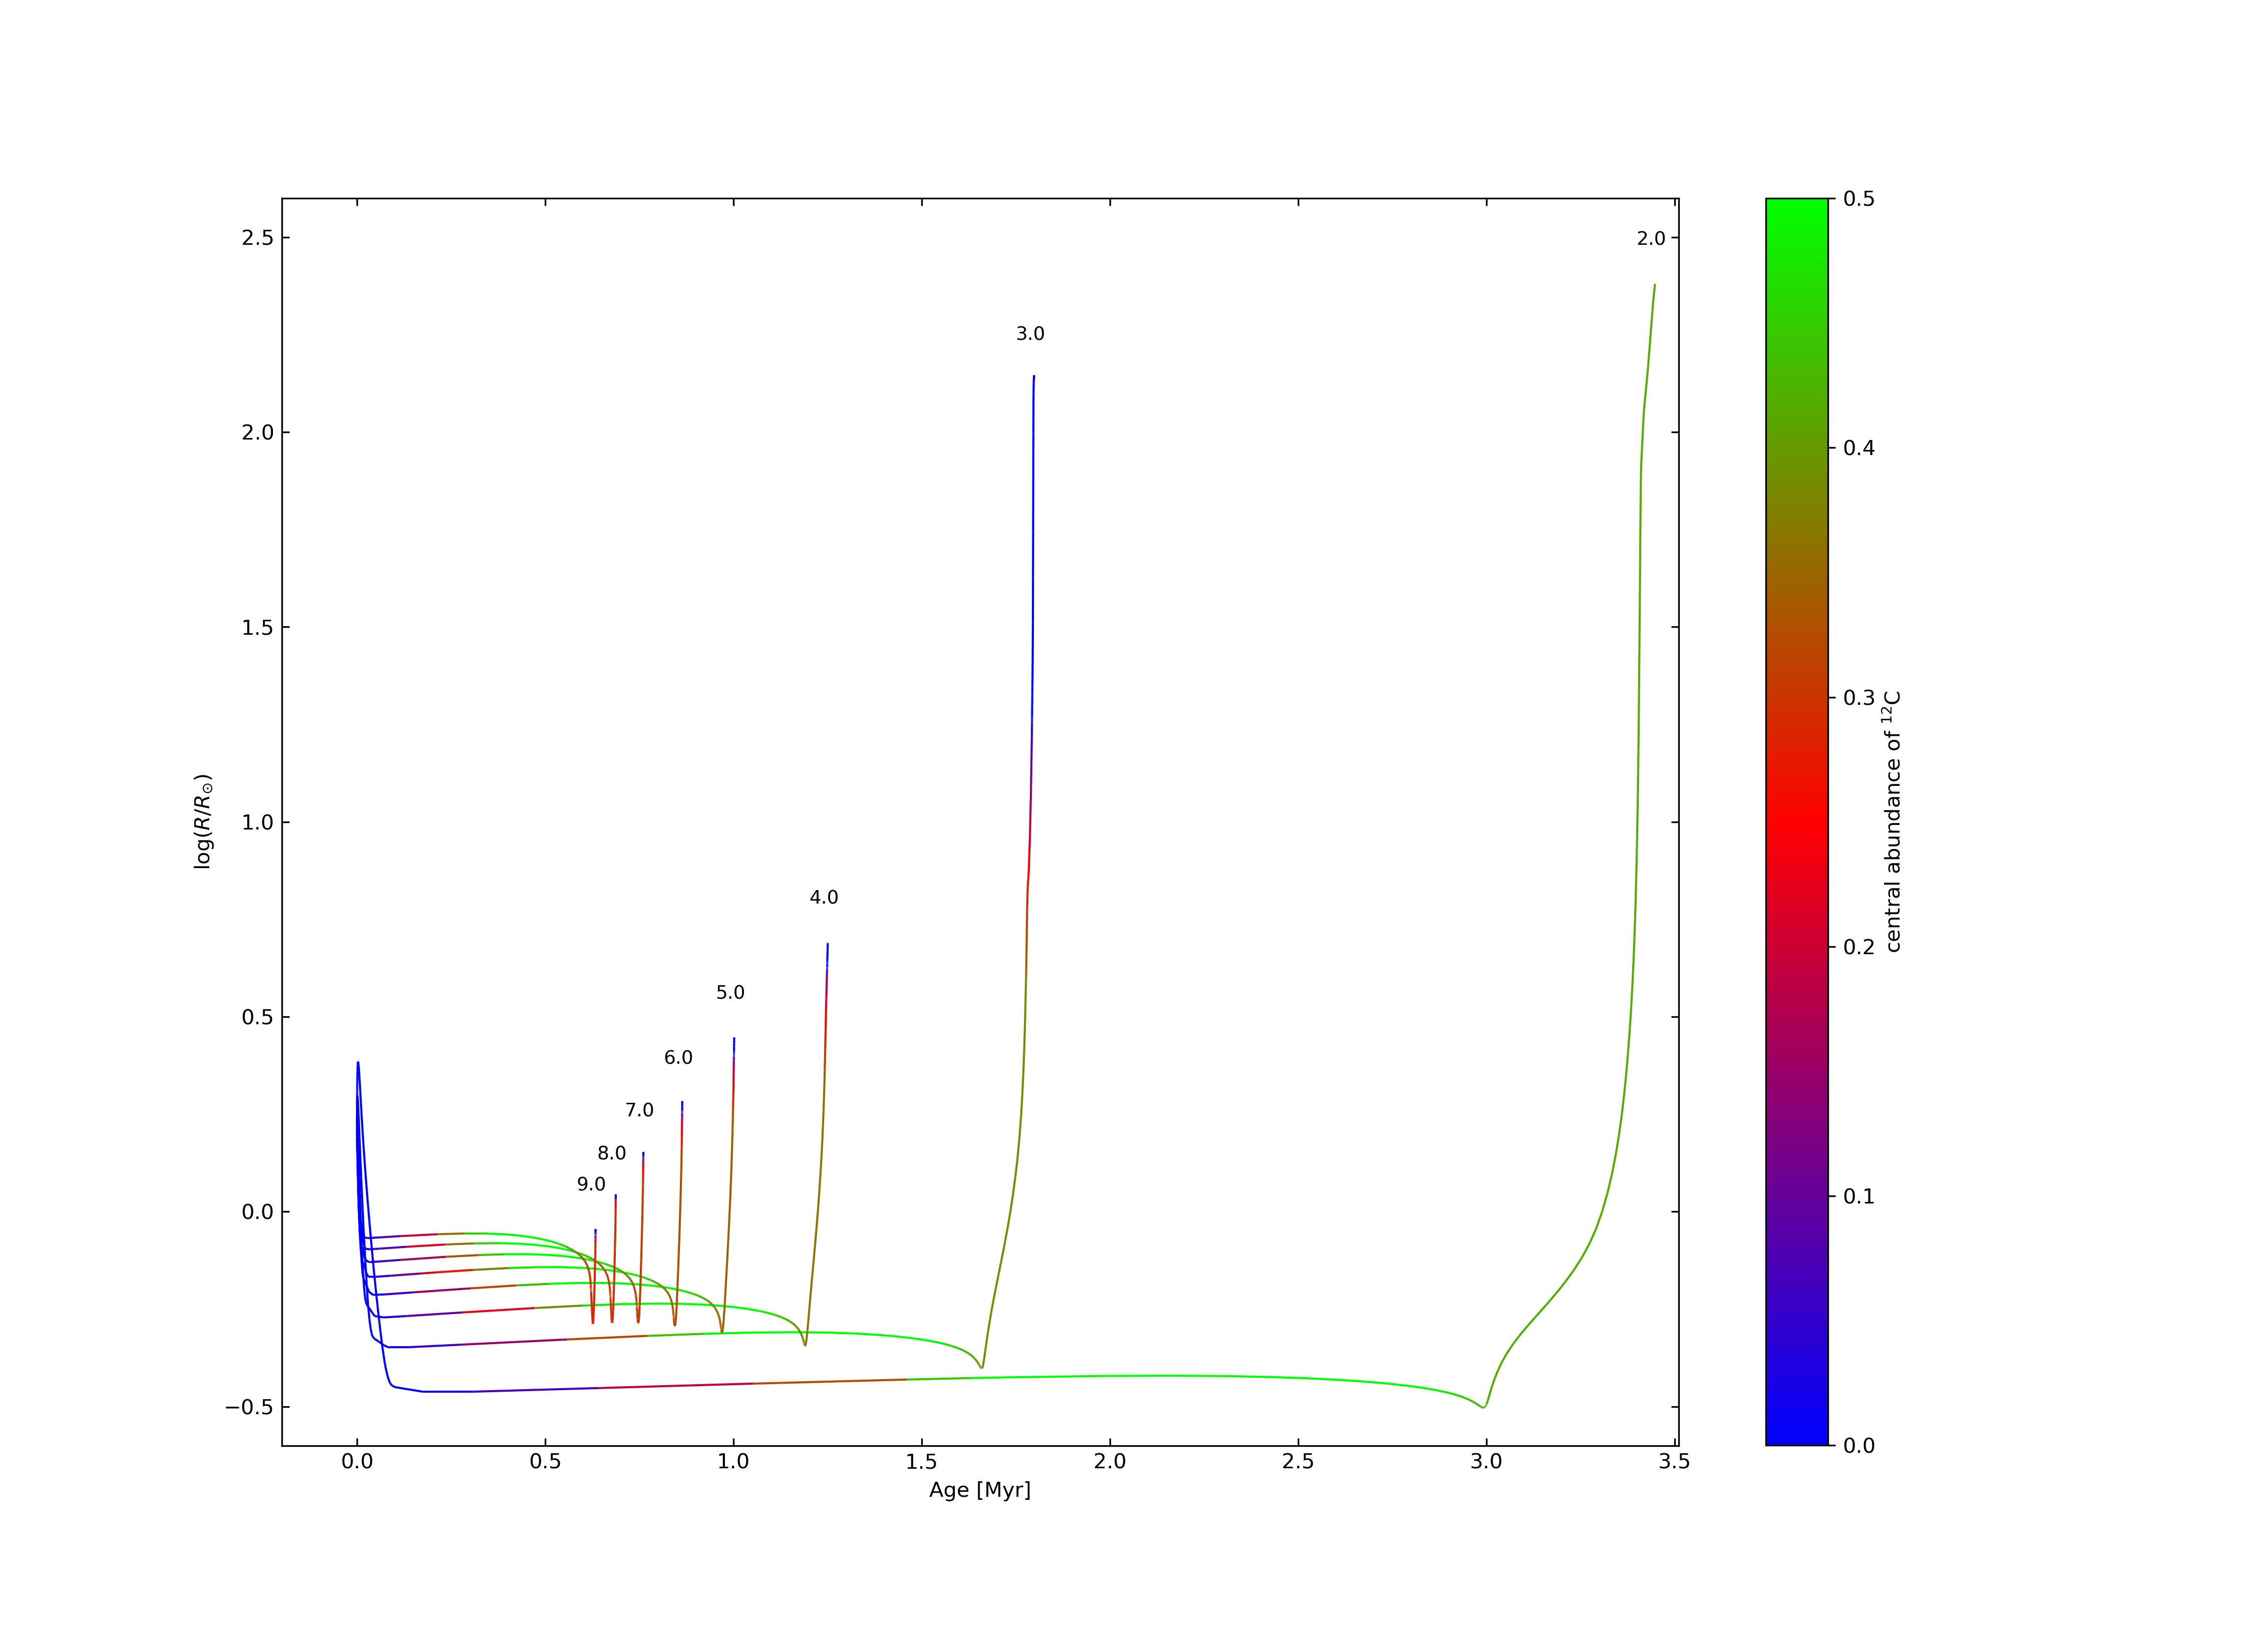
\includegraphics[scale=0.4]{../figures/chapter3/radius_evolution_gradient.png}
						\caption{Evolution of stellar radii as a function of time. The colour map indicates the evolutionary stage of every helium star in terms of the central abundance of carbon whilst the numbers on top of each curve denote the initial mass of the star.}
						\label{fig:radii_singles}
					\end{figure}
				
				
				\subsection{Abundance profiles}	
			
			
			
			\section{Neutron star + helium star binaries}




\end{document}